\documentclass{beamer}
\mode<presentation>
%\usetheme{Warsaw}

\usepackage{amsmath, amssymb, amsthm, graphicx, enumerate, subfigure}
\usepackage{verbatim}
\usepackage[spanish,mexico]{babel}
\usepackage[utf8]{inputenc}
\usepackage[labelformat=empty]{caption}
\usepackage{pifont}% http://ctan.org/pkg/pifont

\definecolor{green1}{rgb}{0.1,0.5,0.2}
\definecolor{green2}{rgb}{0.9,1,0.9}
\definecolor{green3}{rgb}{0.1,0.3,0.2}
\definecolor{green4}{rgb}{0.9,1,0.9}

\useinnertheme{rectangles}


\setbeamercolor*{Title bar}{fg=white, bg=green1}
\setbeamercolor*{section in head/foot}{bg=green1,fg=white}
\setbeamercolor*{title}{fg=white, bg=green1}
\setbeamercolor*{Location bar}{fg=white,bg=green}
\setbeamercolor*{frametitle}{parent=Title bar}
\setbeamercolor*{block title}{bg=green1,fg=white}
\setbeamercolor*{block body}{bg=green2,fg=green3}
\setbeamercolor*{normal text}{bg=white,fg=green3}
\setbeamercolor*{structure}{bg=white,fg=green1}

\newtheorem{defn}{Definición}
\newtheorem{teo}{Teorema}
\newtheorem{prop}{Proposición}

\newcommand{\R}{\mathbb{R}}
\newcommand{\cmark}{\ding{51}}
\newcommand{\xmark}{\ding{55}}

\title{Sistema de recomendación de hoteles similares}
\subtitle{TESIS}
\institute{
\includegraphics[width=0.3\textwidth]{imagenes/logo_ITAM.jpg}\\INSTITUTO TECNOLÓGICO AUTÓNOMO DE MÉXICO}
\author{Felipe Gerard Valdés}
\date{Febrero de 2016}



\AtBeginSection[]
{
	\begin{frame}<beamer>{Agenda}
		\tableofcontents[currentsection]
	\end{frame}
}


\begin{document}

%%%%%%%%%%%%%%%%%%%%%%%%%%%%%%%%%%%%%%%%%%%%%%%%%

\begin{frame}
	\titlepage
\end{frame}

%%%%%%%%%%%%%%%%%%%%%%%%%%%%%%%%%%%%%%%%%%%%%%%%%
\begin{frame}{Agenda}
	\tableofcontents
\end{frame}

%%%%%%%%%%%%%%%%%%%%%%%%%%%%%%%%%%%%%%%%%%%%%%%%%
%%%%%%%%%%%%%%%%%%%%%%%%%%%%%%%%%%%%%%%%%%%%%%%%%
\section{Planteamiento}

%%%%%%%%%%%%%%%%%%%%%%%%%%%%%%%%%%%%%%%%%%%%%%%%%
\begin{frame}{Antecedentes}
	\begin{itemize}%[<+->]
		\item Las ventas de viajes por Internet no tienen asistencia humana
		\item Muchos clientes no conocen los destinos que planean visitar
		\item No basta con permitir que el cliente explore una lista de hoteles
		\item \textbf{Objetivo:} Facilitar la búsqueda del hotel correcto para incrementar las ventas
		\item[$\mathbf{\rightarrow}$] \textbf{Idea:} Para cada hotel, recomendar una lista de hoteles ``similares''
		\item Situación actual:
		\begin{itemize}
			\item Recomendaciones estáticas
			\item Criterio:
			\begin{itemize}
				\item \textbf{Destino:} Usualmente es una ciudad o zona
				\item \textbf{Estrellas:} Categoría del hotel
			\end{itemize}
		\end{itemize}
		\item No está mal, pero ¿se puede mejorar?
	\end{itemize}
\end{frame}

%%%%%%%%%%%%%%%%%%%%%%%%%%%%%%%%%%%%%%%%%%%%%%%%%
\begin{frame}{Análisis de la competencia}
	\begin{itemize}%[<+->] 
		\item Competidores principales: Price Travel, Booking, Despegar, Expedia. Bonus: Trip Advisor
		\item Diversas formas de recomendar:
		\begin{itemize}
			\item Hoteles recientemente vistos: No son recomendaciones genuinas
			\item Hoteles cercanos / en el mismo destino: Estilo y precios pueden ser muy distintos
			\item Recomendaciones con métodos desconocidos (p.ej. ``a otros usuarios les gustó...''): Calidad variable; en general son demasiado rígidos
		\end{itemize}
	\item \textbf{Conclusión:} La competencia deja mucho que desear, pero hay mucho qué aprender
	\end{itemize}
\end{frame}

%%%%%%%%%%%%%%%%%%%%%%%%%%%%%%%%%%%%%%%%%%%%%%%%%
\begin{frame}{\textit{¿Qué queremos?}}
	\begin{itemize}%[<+->] 
		\item Evitar mostrar hoteles demasiado caros
		\item Tomar en cuenta el perfil del hotel
		\item Incorporar información geográfica más detallada que el destino
		\item Que el criterio se adapte a distintos tipos de zonas
		\item Que no se acaben las recomendaciones nuevas (efecto laberinto)
	\end{itemize}
\end{frame}

%%%%%%%%%%%%%%%%%%%%%%%%%%%%%%%%%%%%%%%%%%%%%%%%%
%%%%%%%%%%%%%%%%%%%%%%%%%%%%%%%%%%%%%%%%%%%%%%%%%
\section{Solución}

%%%%%%%%%%%%%%%%%%%%%%%%%%%%%%%%%%%%%%%%%%%%%%%%%
\begin{frame}{Plan de ataque}
	\begin{enumerate}%[<+->] 
		\item \textbf{Precio:} Filtrar hoteles demasiado caros
		\item \textbf{Similitud:} Construir un \textit{criterio integral de similitud}
		\begin{itemize}
			\item Cantidad de servicios
			\item Perfil similar
		\end{itemize}
		\item \textbf{Distancia:} Recomendar hoteles geográficamente cercanos
	\end{enumerate}
\end{frame}

%%%%%%%%%%%%%%%%%%%%%%%%%%%%%%%%%%%%%%%%%%%%%%%%%
\begin{frame}{Precio}
	\begin{itemize}%[<+->] 
		\item Poner hoteles demasiado caros no promueve el interés del cliente
		\item Generalmente más barato es mejor (siempre y cuando tenga la categoría suficiente)
		\item[$\mathbf{\rightarrow}$] Porcentaje máximo arriba del hotel original
		\item Hoteles por encima del precio establecido son invisibles
	\end{itemize}
\end{frame}

%%%%%%%%%%%%%%%%%%%%%%%%%%%%%%%%%%%%%%%%%%%%%%%%%
\begin{frame}{Similitud (P1)}
	\begin{itemize}%[<+->] 
		\item \textbf{Caracterización}
		\begin{itemize}
			\item No bastan las estrellas
			\item Usar información de servicios
			\item Usarla directamente es ruidoso porque no toma en cuenta sustitutos
			\item \textbf{Solución:} Agrupar los servicios en categorías
			\item \textbf{Método:} Manual (criterio de negocio) + aglomerado jerárquico
		\end{itemize}
	\end{itemize}
\end{frame}

%%%%%%%%%%%%%%%%%%%%%%%%%%%%%%%%%%%%%%%%%%%%%%%%%
\begin{frame}{Similitud (P2)}
	\begin{itemize}%[<+->] 
		\item La similitud se puede dividir en dos aspectos básicos
		\item \textbf{Servicios:}
		\begin{itemize}
			\item Al menos ciertos servicios (~ estrellas)
			\item Los servicios faltantes restan similitud
			\item Los servicios extras no se penalizan
		\end{itemize}
		\item \textbf{Perfil:}
		\begin{itemize}
			\item Hoteles del mismo estilo
			\item Misma proporción de cada categoría
			\item Ignorar la cantidad de servicios
			\item Podría dar hoteles más sencillos o más lujosos
		\end{itemize}
	\end{itemize}
\end{frame}

%%%%%%%%%%%%%%%%%%%%%%%%%%%%%%%%%%%%%%%%%%%%%%%%%
\begin{frame}{Similitud (P2)}
	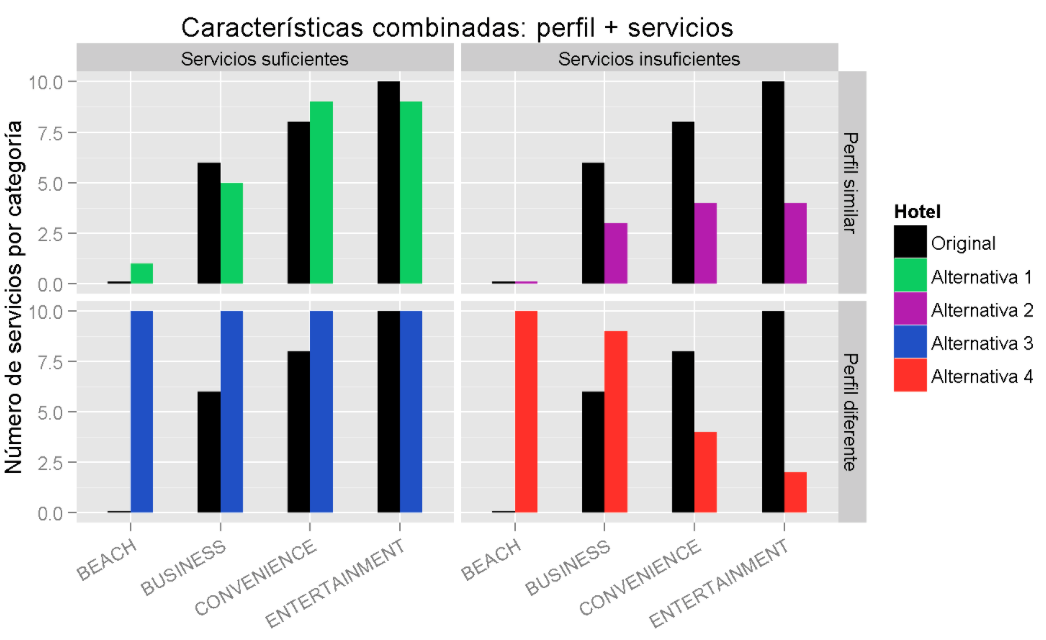
\includegraphics[width=\textwidth]{imagenes/similitud.png}
\end{frame}


%%%%%%%%%%%%%%%%%%%%%%%%%%%%%%%%%%%%%%%%%%%%%%%%%
\begin{frame}{Similitud (P3)}
	\begin{itemize}%[<+->] 
		\item Medida de similitud de servicios: Calidad mínima
		\item Medida de similitud de perfil: Proporciones de servicios
		\item Medida de similitud final:
		\begin{itemize}
			\item Capturar ambos efectos
			\item Promedio ponderado entre ambas medidas
			\item Ponderación de acuerdo a la variabilidad de cada una (PCA)
		\end{itemize}
		\item ¿Por qué no diferencia absoluta?
		\begin{itemize}
			\item Es muy agresiva
			\item No es ajustable
		\end{itemize}
	\end{itemize}
\end{frame}

%%%%%%%%%%%%%%%%%%%%%%%%%%%%%%%%%%%%%%%%%%%%%%%%%
\begin{frame}{Distancia}
	\begin{itemize}%[<+->] 
		\item Hoteles cercanos (usando coordenadas)
		\item El significado de ``cerca'' es variable
		\item Se necesita un criterio dinámico
		\item Cuidar que los hoteles distintos no afecten
	\end{itemize}
\end{frame}

%%%%%%%%%%%%%%%%%%%%%%%%%%%%%%%%%%%%%%%%%%%%%%%%%
\begin{frame}{Distancia}
	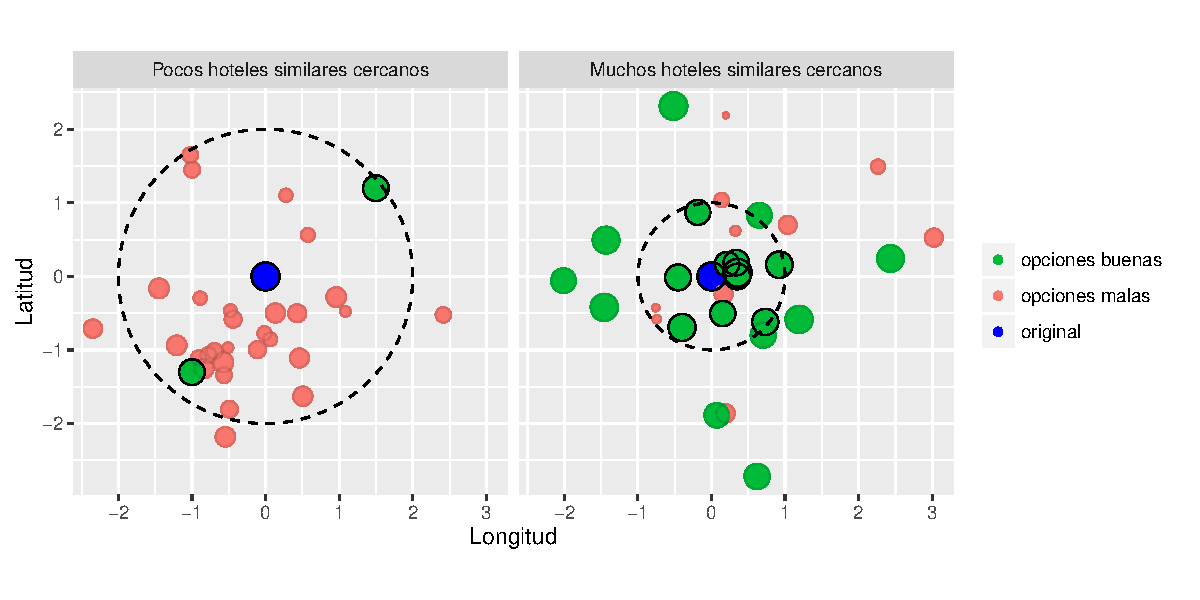
\includegraphics[width=\textwidth]{imagenes/distdin.pdf}
\end{frame}

%%%%%%%%%%%%%%%%%%%%%%%%%%%%%%%%%%%%%%%%%%%%%%%%%
\begin{frame}{Modelo completo}
	\begin{enumerate}%[<+->]
		\item Agrupar los servicios en categorías
		\item Calcular la ponderación entre servicios y perfil
		\item Definir una \textbf{geocerca} (radio de cercanía razonable) alrededor de cada hotel
		\begin{itemize}
			\item Ignorar hoteles caros (precio de largo plazo)
			\item Acumular una cantidad de similitud (mayor peso a hoteles parecidos, menor a los diferentes)
		\end{itemize}
		\item Recomendar dentro de la geocerca de acuerdo a la \textbf{similitud}
	\end{enumerate}
\end{frame}

%%%%%%%%%%%%%%%%%%%%%%%%%%%%%%%%%%%%%%%%%%%%%%%%%
%%%%%%%%%%%%%%%%%%%%%%%%%%%%%%%%%%%%%%%%%%%%%%%%%
\section{Implementación}

%%%%%%%%%%%%%%%%%%%%%%%%%%%%%%%%%%%%%%%%%%%%%%%%%
\begin{frame}{Arquitectura: SQL + \texttt{R}}
	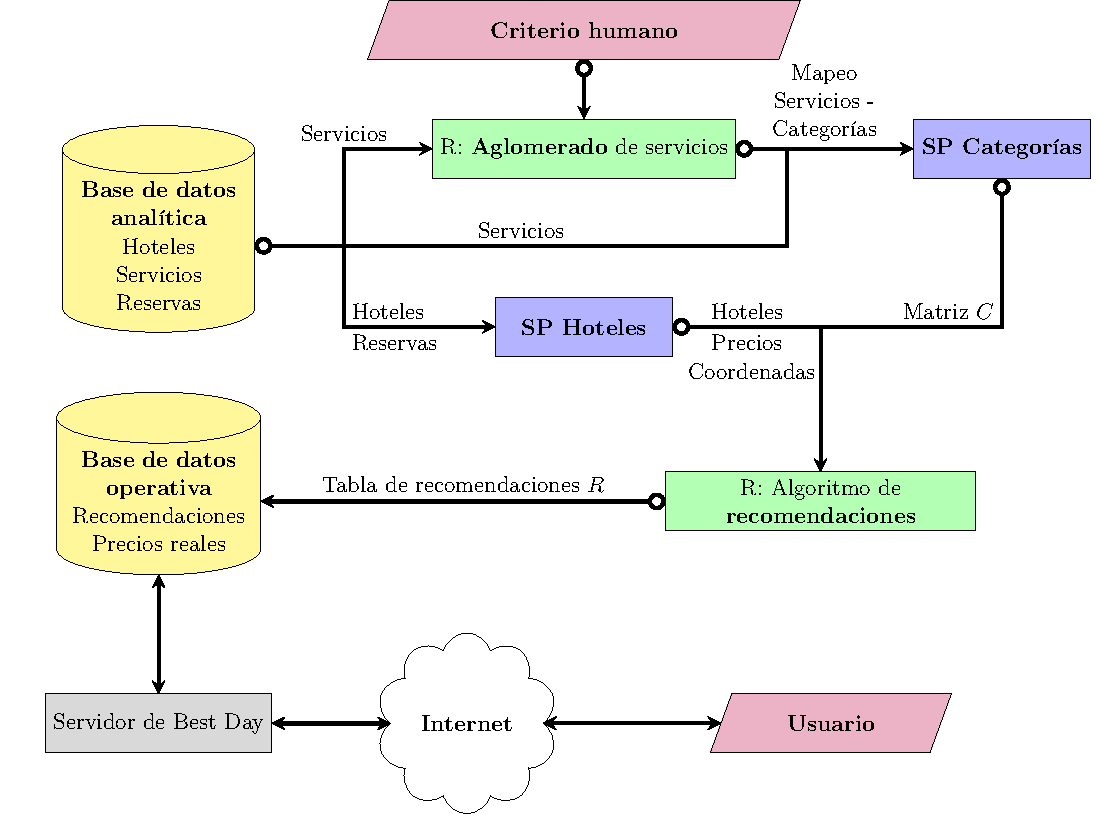
\includegraphics[width=\textwidth]{imagenes/flowchart.pdf}
\end{frame}

%%%%%%%%%%%%%%%%%%%%%%%%%%%%%%%%%%%%%%%%%%%%%%%%%
%%%%%%%%%%%%%%%%%%%%%%%%%%%%%%%%%%%%%%%%%%%%%%%%%
\section{Desempeño}

%%%%%%%%%%%%%%%%%%%%%%%%%%%%%%%%%%%%%%%%%%%%%%%%%
\begin{frame}{Desempeño teórico (antes)}
	\begin{figure}
		\centering
		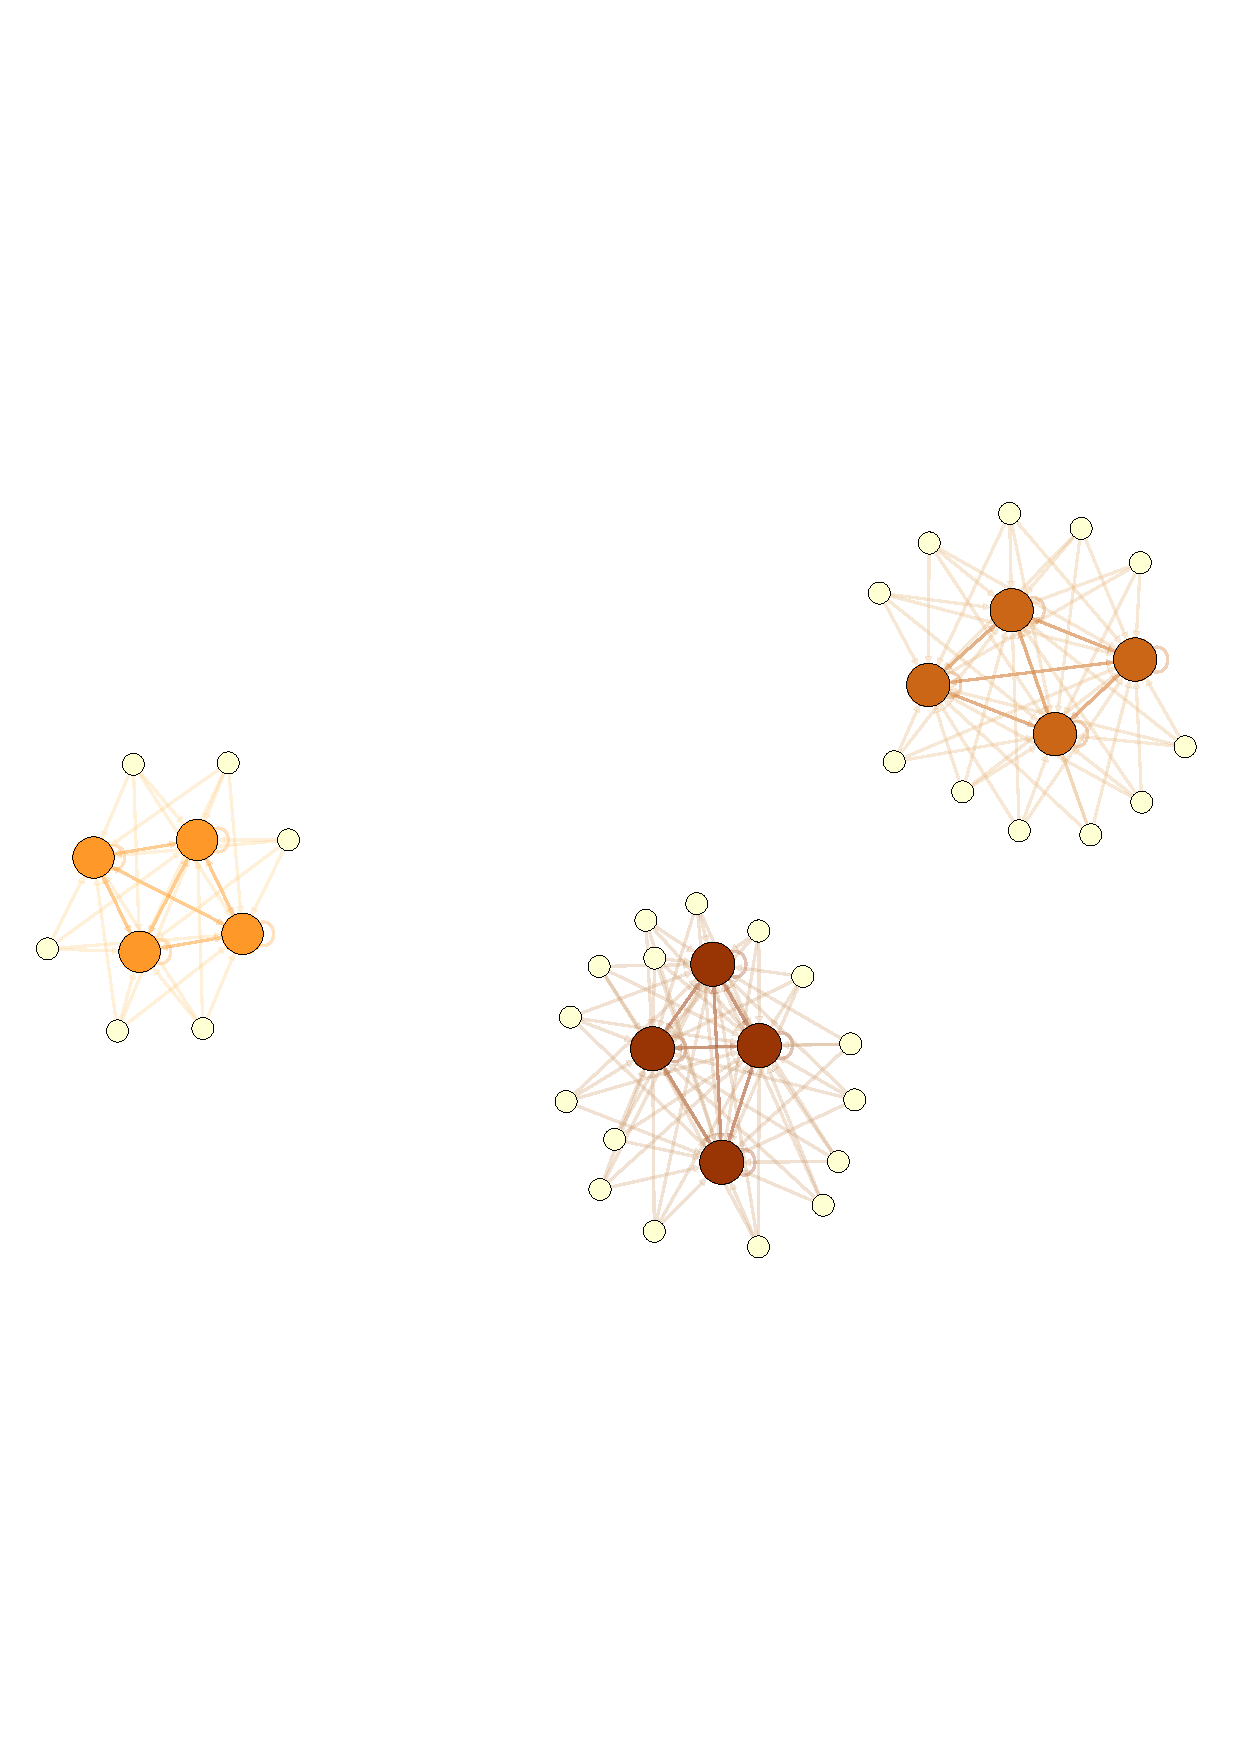
\includegraphics[width=0.6\textwidth, clip = true, trim = 0 0 0 80]{imagenes/disconexo.pdf}
	\end{figure}
\end{frame}

%%%%%%%%%%%%%%%%%%%%%%%%%%%%%%%%%%%%%%%%%%%%%%%%%
\begin{frame}{Desempeño teórico (después)}
	\begin{figure}
		\centering
		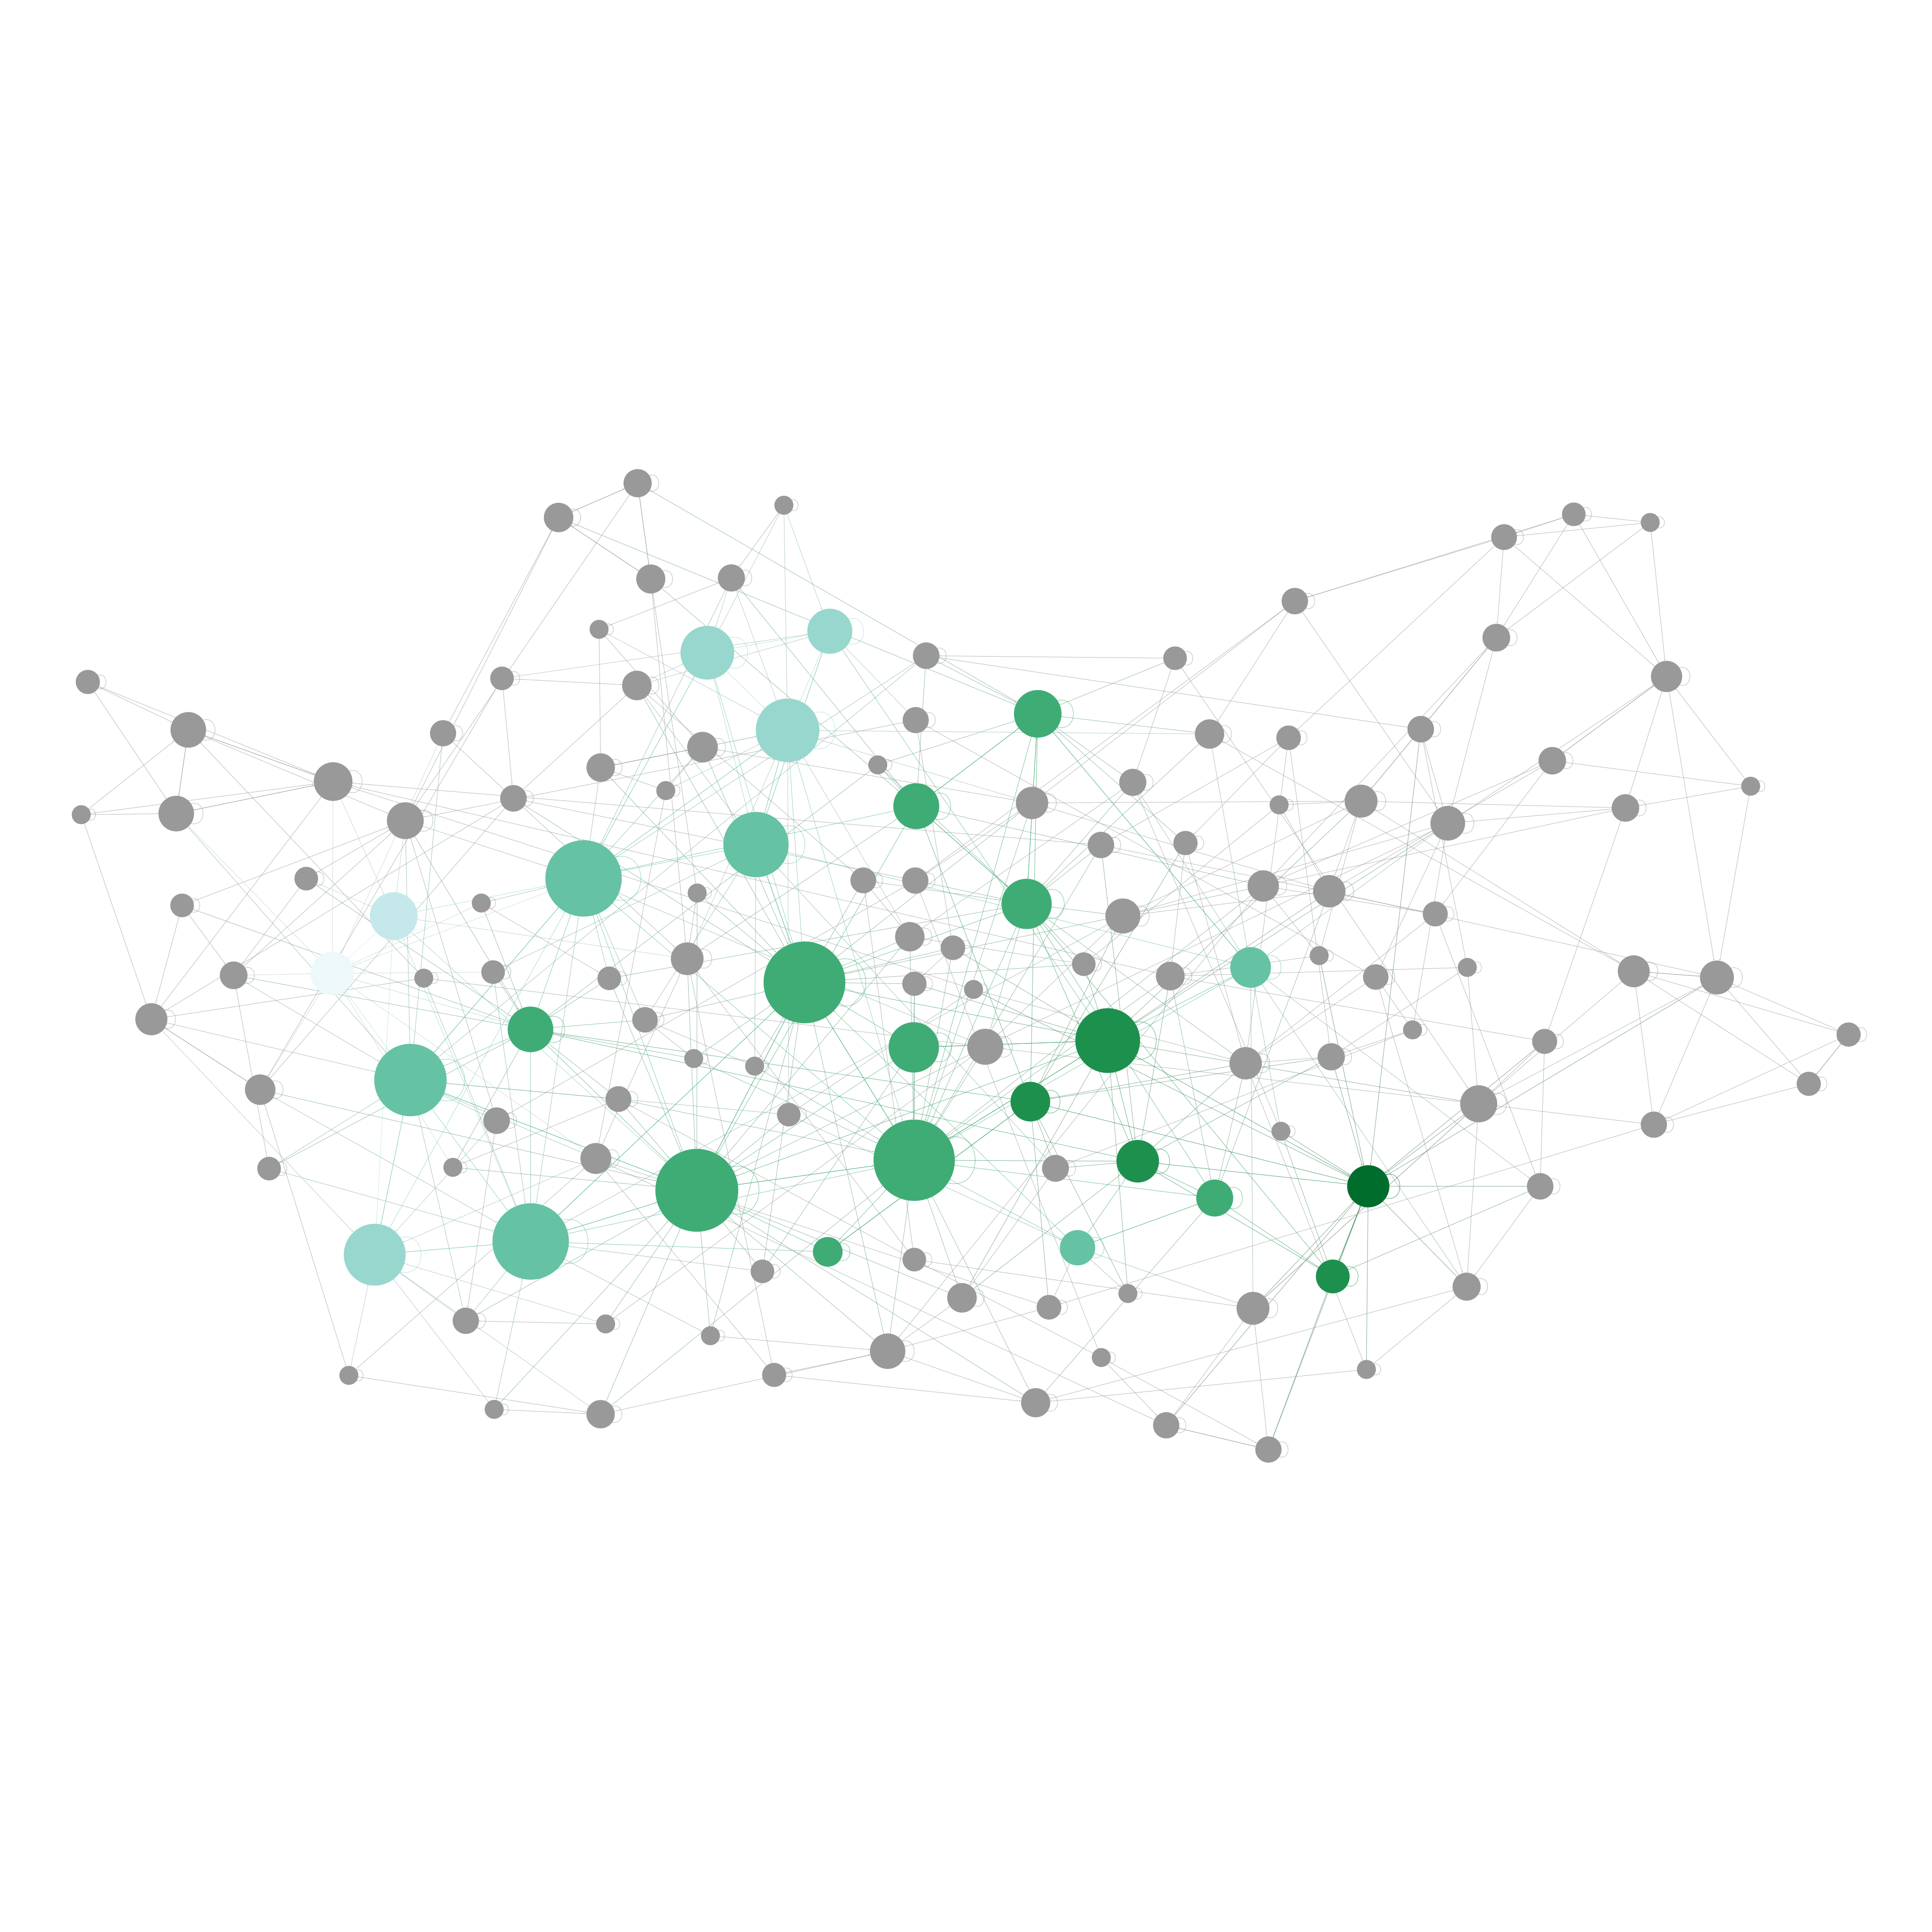
\includegraphics[width=\textwidth, clip = true, trim = 0 0 0 500]{imagenes/cancun_laquinta2.png}
	\end{figure}
\end{frame}

%%%%%%%%%%%%%%%%%%%%%%%%%%%%%%%%%%%%%%%%%%%%%%%%%
\begin{frame}{Desempeño de la página}
	\begin{figure}
		\centering
		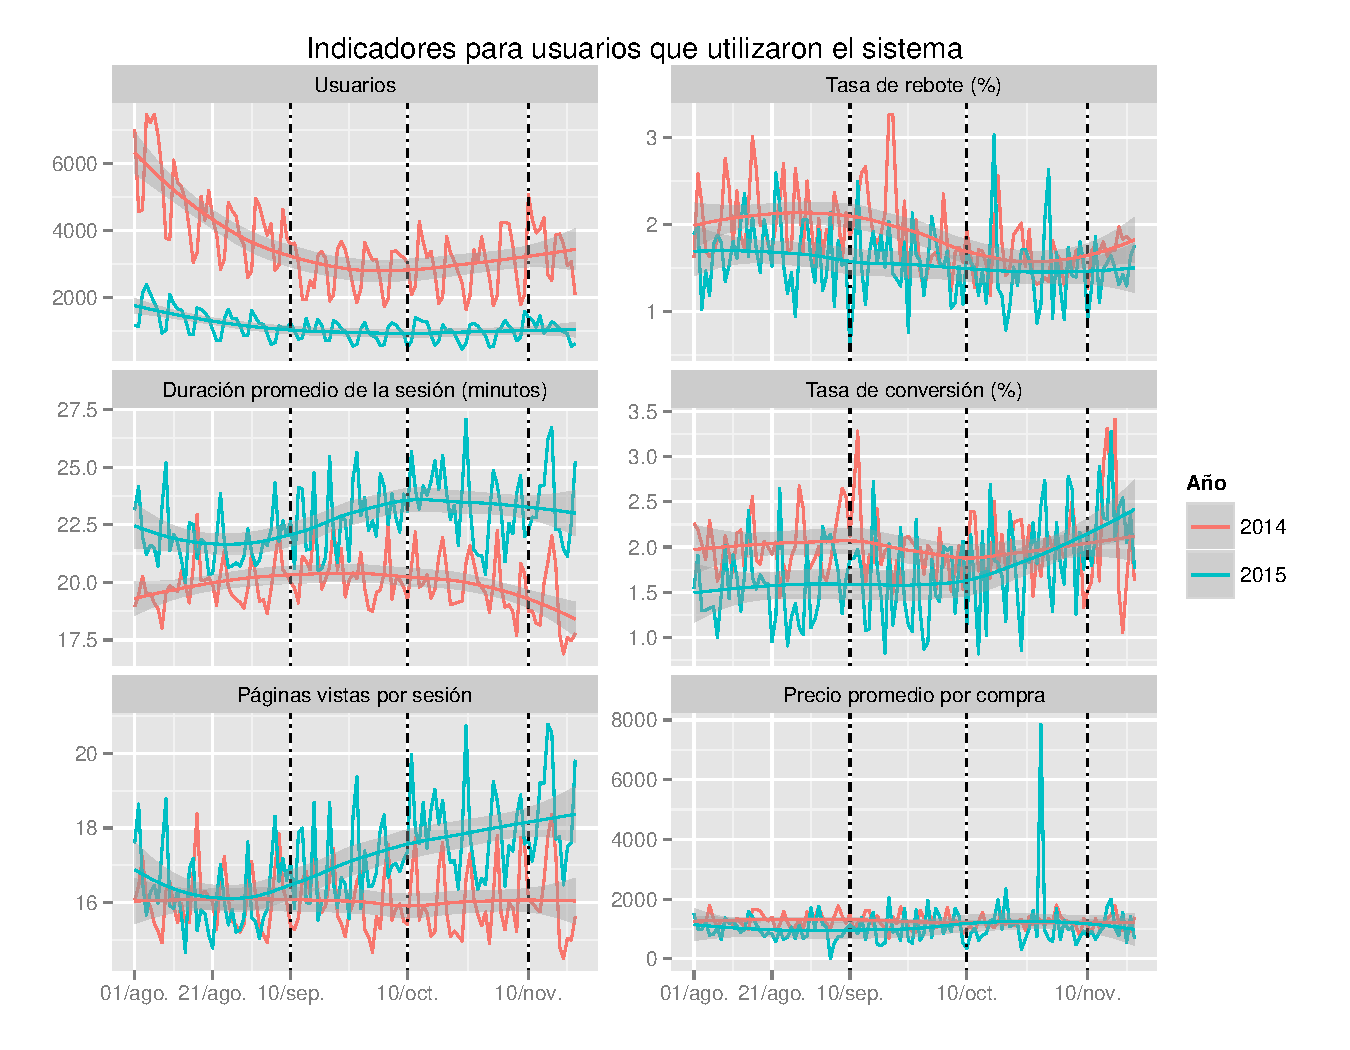
\includegraphics[width=0.85\textwidth]{imagenes/analytics_2015nov23.pdf}
	\end{figure}
\end{frame}

%%%%%%%%%%%%%%%%%%%%%%%%%%%%%%%%%%%%%%%%%%%%%%%%%
\begin{frame}{Conclusiones}
	\begin{itemize}
		\item \textbf{Teóricas:}
		\begin{itemize}
			\item Mejores cualidades: \textbf{precio}, \textbf{distancia}, \textbf{similitud}
			\item La red de recomendaciones está mejor conectada
			\item Mayor \textbf{flexibilidad}: se puede cambiar de categoría gradualmente
		\end{itemize}
		\item \textbf{Prácticas:}
		\begin{itemize}
			\item Impacto importante en los clientes que empezaron a utilizar las recomendaciones
			\item \textbf{Mayor uso} una vez que se utiliza el sistema
			\item Con más tiempo la \textbf{conversión} empezó a aumentar
			\item No hay aumento de entradas (diseño y posición)
		\end{itemize}
		\item \textbf{Trabajo futuro:}
		\begin{itemize}
			\item Precio dinámico, filtro de precio en forma de ``U''
			\item A/B testing
			\item Mayor periodo de observación
		\end{itemize}
	\end{itemize}
\end{frame}




\end{document} 

















